\documentclass[12pt]{report}
\usepackage[utf8]{inputenc}
\usepackage[UKenglish]{babel}
\usepackage[margin=1in]{geometry}
\usepackage{amsmath}
\usepackage{graphicx}
\usepackage{mymacros}
\usepackage{setspace}
\onehalfspacing
% for changing font colour
\usepackage[dvipsnames]{xcolor}

\definecolor{darkRed}{RGB}{189, 20, 17} 
\definecolor{darkBlue}{RGB}{3, 45, 171}
\newcommand{\tcr}[1]{\textcolor{darkRed}{#1}}
\newcommand{\tcb}[1]{\textcolor{darkBlue}{#1}}


\title{An Automated Quality Control System for a Novel Production Line}
\author{jh2044}
\date{February 2020}

\begin{document}

\maketitle

\begin{abstract}
    This project aims to survey and analyse Concrete Canvas' new cement \tcr{impregnated cloth} production line in order to identify and characterise the mechanisms responsible for producing faulty material, as well as develop a \underline{specification} for an on-line computer vision based system capable of \underline{accurately} \tcr{identifying} these faults in real-time.
    
    \tcr{need a short paragraph on cement impregnated fabrics}
    
    The new product, CCX, is a \tcr{extruded} plastic  coated two layer stitch-bonded non-woven geo-textile with a cement-sand dry powder \tcr{infill}. \tcr{The/a} critical manufacturing step is a pressurised \tcr{dry} powder injection  through \tcr{280} parallel \tcr{5mm ID} aluminium tubes. This process is highly volatile and tube blockages occur creating regions of critically underfilled material. Additional failure mechanisms within the other manufacturing steps have been identified \tcr{including stitch drops etc}.
    
    \tcr{During the Summer 2019}, a qualitative analysis of the cement injection process was carried out; a number of phenomena were identified as potential indicators of the powder flow state in the tubes. The feasibility of measuring each of these phenomena was compared. A surface profile measurement using a laser profilometer was selected for further development due to its \tcr{WHYYYY}.
    
    An analysis of the manufacturing process was carried out in order to understand the parameters involved in producing the surface profile of the material. Additional failure mechanisms were identified at each step, and the \tcr{effect on the profile} was considered. \tcr{I feel there is more to be said here, maybe about how the analysis took place etc}.
    
    A profilometer test rig was designed \tcr{and built} \tcr{using a cylindrical datum surface with a tangential laser line, maybe more on this} in order to investigate the nature of the material surface profile in a \tcr{range} of samples. A measurement calibration system was developed. \tcr{maybe something about extending this rig to the production line}.
    
    \tcr{Section on experimentation: what was the experimental protocol, what were the aims, what data, results, discussion}
    
    \tcr{Section on future work}
    
    \tcr{Section on conclusions: What did we find out?, how do we know this?}
    
    
\end{abstract}

\tableofcontents

\chapter{Introduction}
    
    Concrete Canvas is a cement impregnated composite geotextile manufacturer. They currently have two products on the market: Concrete Canvas (CC) and CC-Hydro (CCH), both of which utilise an internal spacer fabric that provides a containment void for the cement-sand powder infill. The spacer is costly due to its complicated manufacturing process. In order to enter the low cost geotextiles market, Concrete Canvas are developing a new alternative product, CCX. CCX does not include the internal spacer in its structure and only uses standard, low-cost components. Instead of the spacer fabric, CCX uses two layers of stitch bonded non-woven fabric web to create a containment void for the cement-sand powder, which is aerated and injected into the void through an array of pressurised lances.
    
    CCX is in a late \tcr{the last?} stage of development, with the final production line currently being designed, constructed and tested. The development of the final line is split into three phases: web stitching, powder injection and plastic coating with a staggered \tcr{staggered or parallel??)} development timeline across the three phases. This parallel development approach allows previous sections of the line to be tested and improved while also allowing later sections to be implemented at the same time. Additionally, line testing data is heavily relied upon in order to direct the improvement of existing sections of the line. A wide range of operating parameters are recorded during test runs of the line as well as data from destructive testing of the produced material, \tcr{but no unified framework exists to facilitate the data analysis required to optimise these parameters to produce better quality material.} \tcb{I'm trying to say that there is not much organisation of test data all together, it's all over a bunch of excel spreadsheets at the moment}. 
    
    \section{Project Motivation}
        An unexpected issue arose during the production line development with the powder injection lances becoming blocked and thus not filling the containment void sufficiently with powder, creating critically weak material. In order to unblock the injection lances, a motor controlled impulse hammer was developed to strike the lances periodically. Concerns were raised about the potential of lance fatigue being caused by the hammer impacts, so a proposal to investigate measurement systems to detect lance blockages was made with the aim of allowing the frequency and magnitude of hammer impacts to be reduced. \tcr{A preliminary investigation was carried out on site at Concrete Canvas during the Summer before the project proper began.}\tcb{(THIS IS DEFINITELY JANK, BUT NEEDS TO BE SAID SOMEHOW)}.
        
        The preliminary investigation resulted in the creation of a number of prototype systems to measure various aspects of the production line in order to infer the lance flow states. The most promising system was a laser-line projection onto the rear surface of the material web passing over a fixed roller with a video camera to reveal the surface profile. During the investigation, other issues with the existing production line became apparent; this suggested that a further investigation of the whole production line would be needed to better understand the processes involved in producing the final material, and to consider ways of controlling and optimising the product quality. 
        
        Effective control and optimisation of the quality of a manufactured product is essential in ensuring its success: a guarantee must be provided that a product will behave according to its performance specification; and by optimising the production parameters, both the quantity of wasted material can be reduced and the product performance enhanced.


    \section{Literature Review}
        The manufacture of geotextiles is a broad field with many techniques and processes involved in the production of several families of geotextiles \cite{berube2016manufacturing} with different material characteristics suited to wide range of applications in civil engineering projects \cite{ingold2013geotextiles}. Concrete Canvas specialises in the manufacture of composite geotextiles, which involves the combination of geotextiles and other components to produce a geotextile with more desirable characteristics than the individual components alone.
        
        Research has been carried out into the development of low-cost laser profilometers, similar to the prototype developed to observe the CCX surface profile such as a soil surface laser scanner which included an effective non-linear calibration scheme and extensive system performance assessment \cite{Darboux2003}, as well as a fabric wrinkle detection system which used a laser-line profilometer and statistical signal analysis to automatically grade fabric smoothness, including variation of beam incidence angle to optimise the system accuracy-resolution trade-off and profile curve fitting to remove systematic error \cite{Xu1998}.
        
        There is extensive research in the field of automatic defect detection in fabric manufacturing processes: many of the systems employ computer vision based techniques to identify the defects \cite{kumar2008computer}, such as a novel approach that estimates the fractal dimension of surface images \cite{conci1998fractal}. Approaches have been developed that use simple bilevel thresholding of images to detect very high-contrast defects \cite{stojanovic2001real}\cite{norton1993machine}, as well as more involved signal analysis of small regions of the incoming images \cite{zhang1995fabric}\cite{huart1994integration}\cite{abou2008line}. Many systems use neural networks to characterise detected defects \cite{stojanovic2001real}\cite{wong2009stitching}\cite{karayiannis1999defect} computed separately from the less computationally expensive direct statistical approaches used for real-time defect detection.
        
        Production Line Quality control systems have been developed to enhance product quality analysis by forming structural equations to represent the manufacturing processes in order to infer unknown operating parameters, and then employing various methods to optimise the product quality such as variance tolerancing \cite{suh2007dynamic},\cite{koo2001variance} and neural-networks \cite{ohshima2000quality}.
        
    \section{Aims and Objectives}
        This project investigated the CCX production line and the material it produces in order to improve the understanding of the manufacturing steps and how each one develops the material characteristics. The investigation broke down each step in the production process and established its operating mechanism, parameters that effect its operation, and also determine existing issues that result in the production of defective material. It also explored and compared a range of measurement systems to detect such defective material.
        
        An investigation of the rear surface profile of the material after the powder injection step was carried out in order to determine its key characteristics, and their distributions within both defective and non-defective material samples. Additionally, the prototype laser-line profilometer system created during the preliminary investigation was developed further to include computationally efficient detection of the incident laser line in the video footage and identification of the key characteristics of the estimated surface profile.
        
        A probabilistic model was developed to approximate the generation of the rear surface profile of the material. This model facilitates the automated detection and characterisation of defects that exist in measured material. The system was tested using samples of material both with and without known defects.
        
        A theoretical framework to unify and structure the logging of data taken from production line operation (online parameters) and destructive testing (offline parameters) was devised. The framework associates all measured parameters to the appropriate location on the produced material web, and relates parameters using a hierarchical dependence structure. This framework provides the basis for an analysis of the measured data to maximise produced material quality by optimising the production parameters.
        
        
        
\pagebreak
\chapter{Background}

    \tcr{need a short paragraph on cement impregnated fabrics}
    
    The new product, CCX, is a \tcr{extruded} plastic  coated two layer stitch-bonded non-woven geotextile with a cement-sand dry powder \tcr{infill}. \tcr{The/a} critical manufacturing step is a pressurised \tcr{dry} powder injection  through \tcr{280} parallel \tcr{5mm ID} aluminium tubes. This process is highly volatile and tube blockages occur creating regions of critically under-filled material. Additional failure mechanisms within the other manufacturing steps have been identified \tcr{including stitch drops etc}.
    
    \tcb{who is concrete canvas? where are they based?}
    \tcb{what is a geotextile? What materials does this include?}
    
    
    \section{Concrete-Fabric Composites}
    \tcr{Geotextile materials have a wide range of applications: ditch lining, bund lining, erosion protection, the list goes on}
    Concrete Canvas and CC-Hydro \tcb{why two, what are the differences, similarities?}
    
    \section{CCX Overview}
        \subsection{Material}
            need to descrube what the material is, what it is made up of, it's known properties, it's projected property targets. Individual component properties, manufacturing etc.
            Non-woven surface
            \addfigured{.5}{figures/background/1x_HH_surface.jpg}{HH (upper?) non-woven surface}{hh_1x}
            \addfigured{.5}{figures/background/1x_HI_surface.jpg}{HH (lower?) non-woven surface}{hi_1x}
            \addfigured{.5}{figures/background/5x_HH_calen.jpg}{HH (upper?) non-woven surface 5x microscopic view}{hh_5x}
            \addfigured{.5}{figures/background/5x_HI_calen.jpg}{HI (lower?) non-woven surface 5x microscopic view}{hi_5x}
        \subsection{Production Line}
            overview
            
            this section will provide the background information as to what technology and systems are in place to make the material. mechanical process descriptions etc. 
            \addfigured{1}{figures/background/process_flow_overview.pdf}{production line process flow overview}{ccx_process_overview}
            \addfigured{1}{figures/background/CX02_V03_side_drawing.png}{production line physical overview}{ccx_line_overview}
            unwind stations 
            \addfigured{0.8}{example-image-a}{image of yarn unwind creole}{yarn_creole}
            \addfigured{0.8}{example-image-b}{image of unwind stand}{nw_unwind_stand}
            \addfigured{0.8}{example-image-c}{image of unwind stitching stand}{nw_inline_stitching}
            \addfigured{0.8}{example-image-a}{diagram to describe Maliwatt Stitchithing}{matliwatt_stitch}
            \addfigured{0.8}{example-image-b}{image to describe lances and injection}{cement_injection}
            \addfigured{0.8}{example-image-c}{image to describe extraction box}{extraction_box}
            something about accumulation here
            
            something about machine parameters, on a large scale (lengths, widths, speeds. But at the scale of the whole line. Individual parameters are included in the full analysis.
            \addfigured{0.8}{example-image-c}{table of machine parameters}{machine_parameters}

\chapter{9}
    
    During the development of the production line, defects were found in samples of produced material. It is essential for any defects in a manufactured product to be carefully controlled for to guarantee its quality. This chapter will detail the investigation carried out to identify the types of defects that appear in the material, as well as their causal pathway. It will discuss the considerations of what measurements of the line could be made to identify these defects and the process behind the decision to use a line laser profilomter with digital camera system to detect the faults.
    
    
           
\chapter{Production Line Investigation}
    A qualitative investigation of the CCX production line was carried out in order to better understand the processes and variables involved in producing the final product. The key aim of the investigation was to identify the mechanisms responsible for producing defective material, and what additional on-line measurements could be taken in order to identify such defects automatically.
    
    \section{Injection Lance Blockage}
        \addfigure{1}{figures/line_investigation/injection_side_cutaway.pdf}{Injection Process Diagram}{injection_side}
        \addfigure{1}{figures/line_investigation/injection_front.pdf}{Injection Drawing}{injection_front}
        
    \section{Defect Generation}
        
    \section{Defect Characterisation}
    

\chapter{Surface Profile Measurement}
    Following the 
    \tcr{all notation is a work in progress and definitely subject to change and hopefully my explanation will solidify as I actually work out what I'm doing}
    \section{Raw Laser Line Image Processing}
        \begin{figure}[ht!]
            \centering
            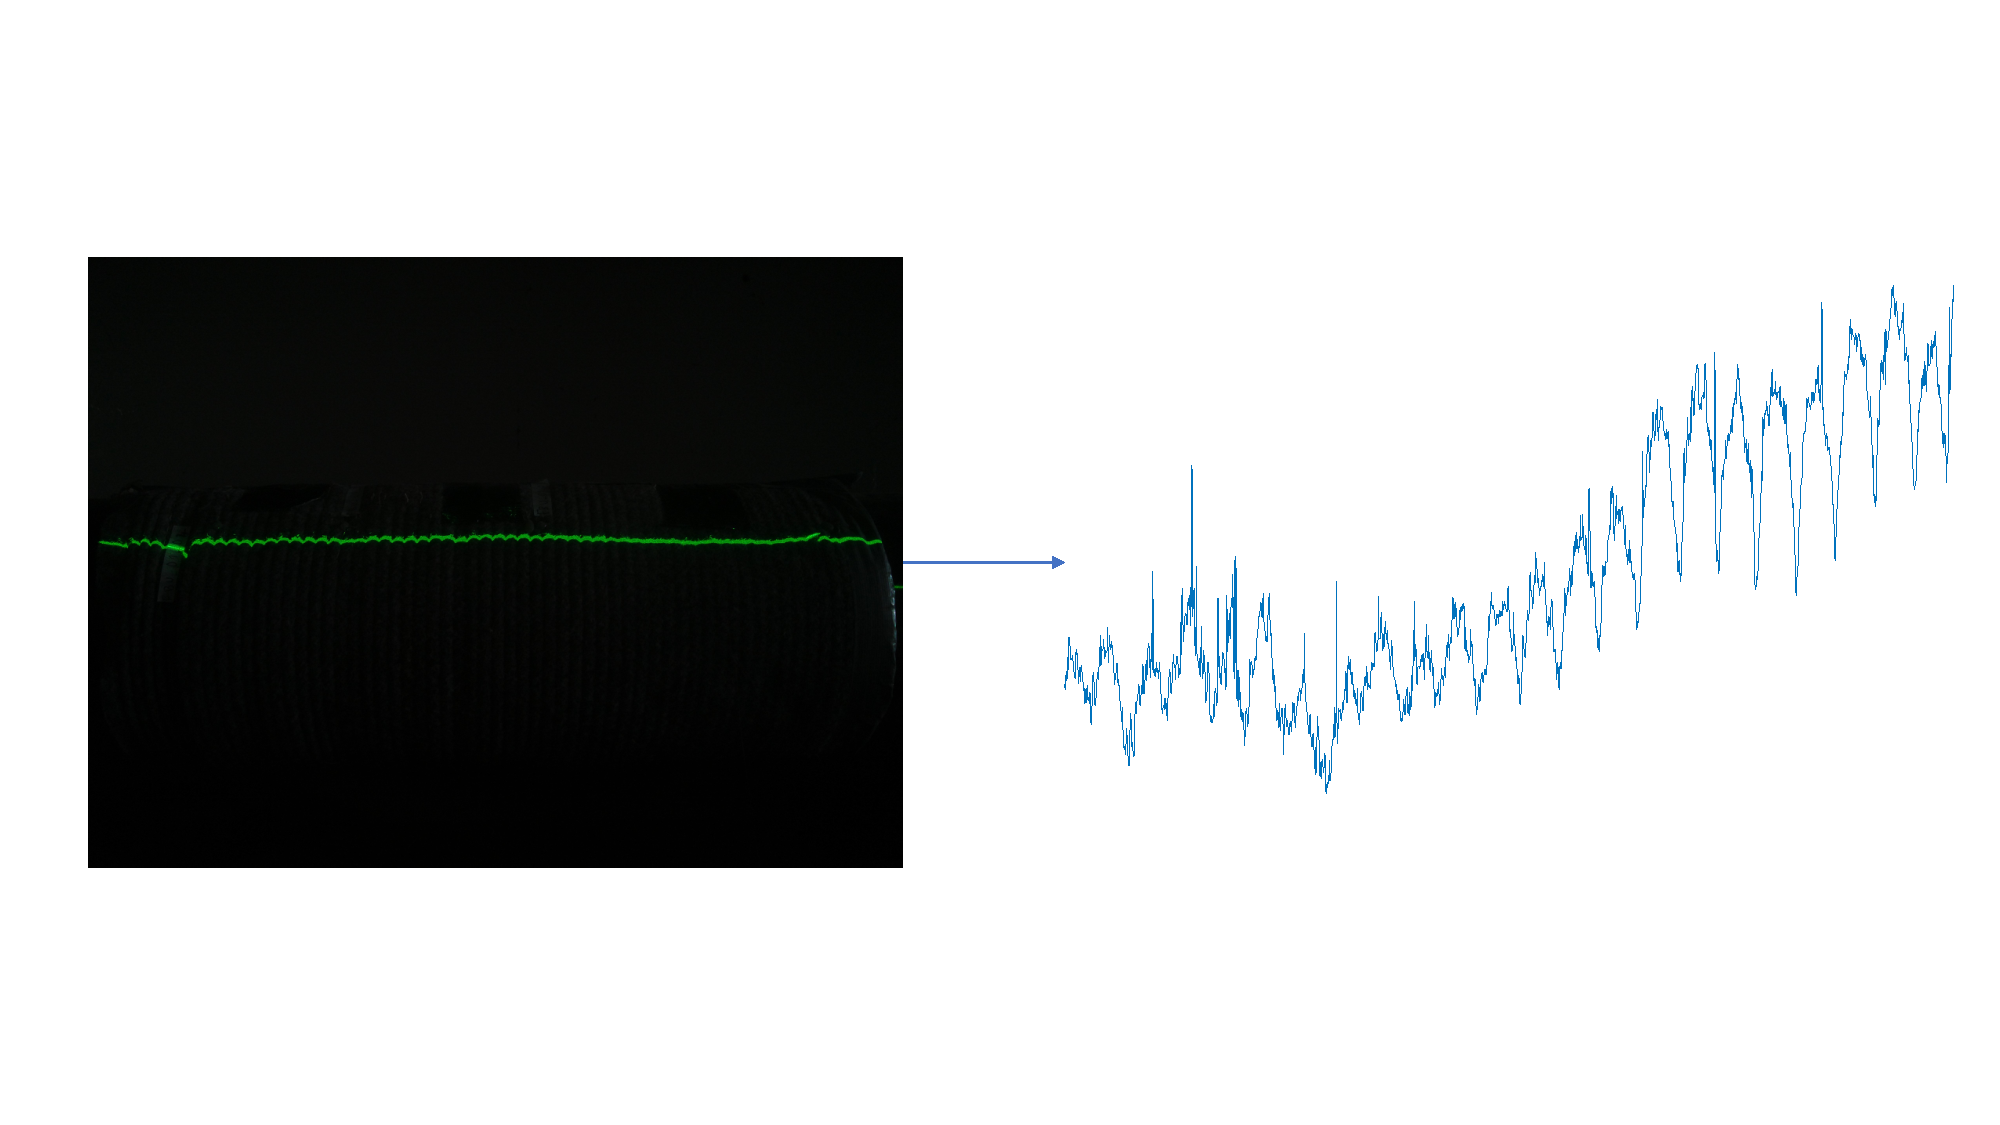
\includegraphics[width=\textwidth,trim={0 5cm 0 5cm},clip]{figures/profile_measure/temp_height_measure.pdf}
            \caption{Raw Laser Line Image Processing}
        \end{figure}
        This process transforms each image into a calibrated estimate of the material surface. In summary:
        
        \begin{itemize}
            \item Crop image to relevant region
            \item Threshold image for laser light
            \item Compute estimate for the laser height at each pixel column by comparing the light intensities
            \item Transform camera coordinates into world coordinates.
            ie $(\text{column}, \text{row}) \rightarrow (x',z')$. This requires taking into account the laser plane to camera geometry, and a simple grid calibration in the plane of the laser can be used to generate static calibration constants.
            \item transform world coordinates into material coordinates: $(x',z') \rightarrow (x,y,z)$. This requires consideration of the laser plane to material surface geometry and a correspondence between the image acquisition time and the roller movement speed/position. \tcr{Note, we will likely average over the displacement of each measurement in the longitudinal ($y$) direction for simplicity}
        \end{itemize}
    
    \section{Profile Parameterisation}
        \begin{figure}
            \centering
            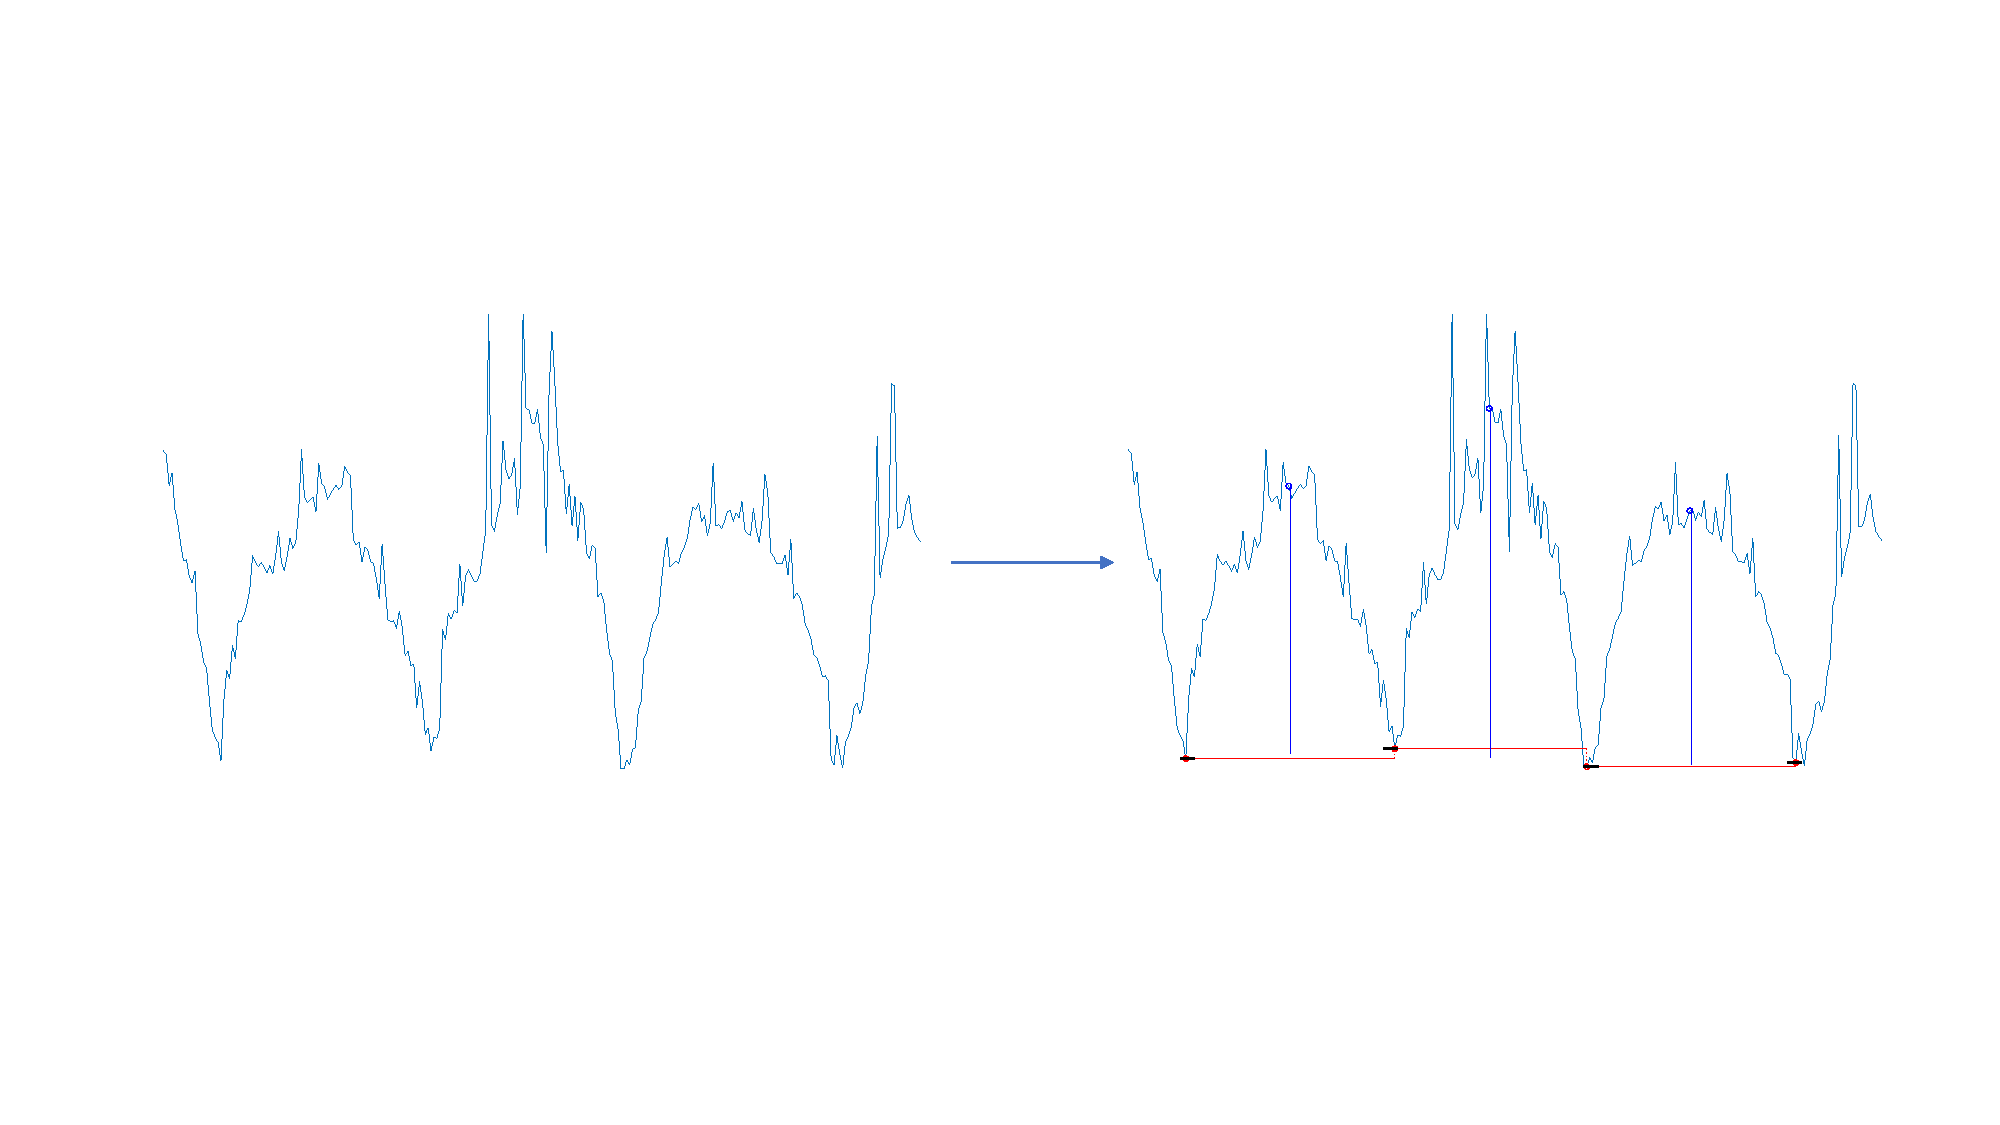
\includegraphics[width=\textwidth,trim={0 5cm 0 5cm},clip]{figures/profile_measure/temp_parameterise.pdf}
            \caption{Profile Parameterisation}
        \end{figure}
        This process transforms each set of surface measurement points into a set of parameters corresponding to the bumps/stitch tracks on the surface.
        
        \begin{itemize}
            \item Compute stitch track locations 
            \item compute observed bump parameters $\pmb{\theta}^*_{ij}$
        \end{itemize}
        
        note that $\pmb{\theta}_{ij}$ corresponds to the $i$-th bump along the surface, at the $j$-th location in the longitudinal direction. also $\pmb{\theta} = [\theta_1,\theta_2,\ldots ,\theta_n]^T$ as some vector of parameters.
        
        The parameters describe elements of the bumps such as:
        \begin{itemize}
            \item width (trough-trough $x$ distance)
            \item relative height (trough-peak) height
            \item absolute height ($z$ position of troughs/peaks)
            \item curvature
            \item trough height change (trough-trough $z$ distance)
            \item surface fluffiness
        \end{itemize}
         
        This significantly reduces the size of the data-set by drawing out useful features of the profile that give an indication of the state of the observed profile in terms of its material characteristics. A careful choice of parameters is required in order to give an optimal trade-off between computational complexity and accuracy. If the parameterisation is too simplistic, it may cause not convey the required information about the surface, but too complex and the computation will be too costly to achieve a sufficiently high frame-rate.
        
        \tcr{note also that the further discretisation of the surface achieved by paramterisation does not necessarily have to be confined to bumps, but currently this seems like the most sensible unit size due to each bump containing all of the information of the material at that local region}
        
        \subsection{Current parameterisation}
            \begin{figure}
                \centering
                \includegraphics[width=0.6\textwidth,trim={8cm 25cm 8cm 28cm},clip]{figures/profile_measure/IMG_20200414_092202.jpg}
                \caption{Current Bump parameterisation}
            \end{figure}
            The current parameterisation transforms any given bump to the following parameterisation (See figure above):
            \begin{itemize}
                \item $\theta_1$: absolute left trough height
                \item $\theta_2$: bump width
                \item $\theta_3$: trough height difference
                \item $\theta_4$: relative height difference from trough average height to height at midpoint of bump 
            \end{itemize}
            \tcr{one key downside to this parameterisation is that it will contain a significant amount of noise from the fluffiness and just assume it is the bump height. A better parameterisation that should not compromise simplicity too much is in the pipeline as this method does not give very good results on the bump relative height front}

\chapter{Automatic Defect Detection}
    \section{Profile Generation Model}
        We propose that $\pmb{\theta}$ (some bump parameterisation) is a random variable with
            \[ \pmb{\theta} \sim f(\pmb{\beta}) \]
        where $f$ is a probability density function with parameters $\pmb{\beta} = [\beta_1,\beta_2,\ldots,\beta_n]^T$ defined by the profile generating model $\mathcal{M}$.
        We assume that all bumps $\pmb{\theta}$ are independently generated. This assumption greatly simplifies the analysis. It does, however, ignore any possibility of a correlation between bump parameters in a local neighbourhood. We also assume that the parameters $\pmb{\beta}$ are also random variables with an unknown distribution. This allows the underlying generation function to change for different bumps.
        
        \subsubsection{Current Generation Model $\mathcal{M}_1$}
            The current system employs the most simple generation of the parameters which assumes that each element of $\pmb{\theta}$ is generated independently of the others with the following distribution types (the distribution type selection was based on an analysis of the nature of the parameters and also the data coming out of samples, a more convincing argument might be possible):
            \begin{itemize}
                \item $x_1$: normally distributed
                \item $x_2$: normally distributed
                \item $x_3$: normally distributed
                \item $x_4$: generalised extreme value distribution
            \end{itemize}
            each of these distributions have parameters which are contained in $\beta$.
            
            \tcr{The hope is to improve the parameterisation and to get the representation of bump height to be normally distributed as well. it is currently extreme value (long tail) because of the fluffiness generating a very large spread of possible values}
        
    \section{Model Training}
        We have a set of profile bump measurements with parameters $\{\pmb{\theta}^*_1,\ldots,\pmb{\theta}^*_N\}$ used for training model $\mathcal{M}$. In order to train the model, we perform log likelihood maximisation over the model parameters $\pmb{\beta}$:
        
        \[
            \pmb{\beta}^* = \underset{\pmb{\beta}}{\arg\max}\log\mathcal{L}_\mathcal{M}(\pmb{\beta}\mid \{\pmb{\theta}^*_1,\ldots,\pmb{\theta}^*_N\})
        \]
        
        The optimal $\pmb{\beta}^*$ then represents the best generation parameters for the training set. We manually select samples we believe were generated from different regions of the generation space (broadly nominal, stitch fail, unfilled, and different samples with new problems) and train the model for all of these sample types separately. Each of these optimised $\pmb{\beta}^*$ gives a unique generation distribution which represents the type of sample it produces. 
        \tcr{explanation of this bit is not very good, as I'm stumbling over my words}
    
    \section{Inference}
        With some set of trained bump generation parameters $\{\pmb{\beta}^*_1,\pmb{\beta}^*_2,\ldots,\pmb{\beta}^*_m\}$ representing $m$ bump generation categories, we can perform inference of the bump generating category of some test set $\{\pmb{\theta}'_1,\ldots,\pmb{\theta}'_N\}$ by comparing the likelihood that some generation parameters generated the test set:
        
        \[ 
            \mathcal{L}(\pmb{\beta}_k \mid \{\pmb{\theta}'_1,\ldots,\pmb{\theta}'_N\})
        \]
        
        we then conclude that the test set was generated with the parameters with the highest likelihood. Additionally, for the on-line system, to minimise the computational requirements, we only compute the likelihood of the nominal generation parameters given the test set. This will still give an indication of a fault in the material, but will not specify the nature of the fault.
        
    \section{Potential Issues/considerations}
        \subsection{Overfitting}
            Poor choice of $\pmb{\theta}$ may cause the model to train to a very high likelihood for the given training set, but any test set that is asserted to be a member of the same generation category will report a low likelihood of membership. 
        \subsection{Training sample data}
            Given that Concrete Canvas has a very limited knowledge of what is actually `nominal' material, it is challenging to develop a decent training set to represent this. As the currently `nominal' set contains significant parametric variance which may contain unknown faults.
            Also, given the data-set is very small, the training sets may not actually be representative of the full generation space.
        \subsection{Modelling Decisions}
            The current system proposes a `stateless' generation process, but actually there may be significant correlation between generated bumps, both spatially (across the material) and temporally (along the material). 
        \subsection{Parameter Choice}
            By discretising our surface to individual bump units, the implicit assumption is made that the bump units contain all of the relevant information for that region of the surface.
        \subsection{Noise/measurement resolution}
            All testing and development to this point has been done with the very high precision data provided by the static scanner (0.1mm $x$ and $\sim$0.5mm $y$). The minimum required resolution for the online system to draw statistically significant conclusions is unknown
            
\chapter{QC Analysis Parametric Framework}
\chapter{Future Work}
\chapter{Conclusions}

%Sets the bibliography style to IEEE and imports the 
%bibliography file "refernces.bib".
\bibliographystyle{IEEEtran}
\bibliography{references}

\end{document}
